cre\documentclass{article}

\usepackage{amsmath}
\usepackage[utf8]{inputenc}
\usepackage[OT4]{polski}
\usepackage{graphicx}
\usepackage{subcaption}

\title{~Put title here~}
\date{\today}
\author{Adrian Rupala}

\begin{document}
	\pagenumbering{gobble}
	\maketitle
	
	\newpage
	\tableofcontents
	
	\newpage
	\pagenumbering{arabic}
	
	\section{Section}		
	Litwo! Ojczyzno moja! Ty jesteś jak zdrowie. Ile cię trzeba było głucho w jedno i aby w koryta rozlewa. Sędzia, a bij jak mnie polityka nudzi. jeżeli z jego postać tylko chodzić zwykła z Paryża baronem. Gdyby żył dłużej, może zyska bo tak rzadka ciche grusze siedzą. Śród cichej wsi długo dumał, nim stał w kalendarzu można równie kłaść na gości prosi w Tabor w okolicy. i kłopotach, i jakobffy dwa tysiące kroków zamek dziś toczy się pomieszany, zły i słudzy. I przyjezdny gość, krewny pański i niewesoły rozbierał myślą wszystkie Tadeusza wzrok stryja ku studni, której lat kilku dni zbiera na wybór wziął tytuł markiza. Jakoż, kiedy się sam na tyle nauki lękał się, że go miało być chwytny? Więc było głucho w pole psy tuż, i dziwu pobladła. twarz nadobną odgadywać zwykła. Myślił, że słuchał rozmowy grzeczne z Francuzem gada na awanpostach nasz z wojażu upodobał mury tłumacząc, że posiadłość tam pewnie miała wysmukłą, kształtną, pierś powabną suknię materyjalną, różową, jedwabną gors wycięty, kołnierzyk z Wilna, nie wiem, czy moda francuszczyzny! gdy przysięgał na partyję Kusego bez przerwy. \\
		
	'Pójdźże, kiń tę chmurność w głąb flaszy!'
	'Dość gróźb fuzją, klnę, pych i małżeństw!'
	'Pójdź w loch zbić małżeńską gęś futryn!'
	'Filmuj rzeź żądań, pość, gnęb chłystków!'
	'O, mógłże sęp chlań wyjść furtką bździn.'
	'Mężny bądź, chroń pułk twój i sześć flag.'
	'Chwyć małżonkę, strój bądź pleśń z fugi.'
		
	
	\subsection{Subsection}
	Structuring a document is easy.
	
	\subsection{Math stuff}
	
	\begin{equation}
	f(x) = x^2
	\end{equation}
	
	This formula $f(x) = x^2$ is an example.
	
	\begin{equation*}
	1 + 2 = 3
	\end{equation*}
	
	\begin{equation*}
	1 = 3 - 2
	\end{equation*}
	
	\begin{align*}
	1 + 2 &= 3\\
	1 &= 3 -2
	\end{align*}
	
	\begin{align*}
		f(x) & = x^2                     \\
		g(x) & = \frac{1}{x}             \\
		F(x) & = \int^a_b \frac{1}{3}x^3
	\end{align*}
	
	\begin{equation*}
		\begin{matrix}
			1 & 0 \\
			0 & 1
		\end{matrix}
	\end{equation*}	
		
	$\begin{matrix}
		1 & 0\\
		0 & 1
	\end{matrix}$
	
	$\left[
	\begin{matrix}
		1 & 0\\
		0 & 1
	\end{matrix}
	\right]$
	
	$ \left(\frac{1}{\sqrt{x}}\right) $
	
	\subsection{Pictures}
	  This is another subsection.
	  
	\begin{figure}[!ht]
		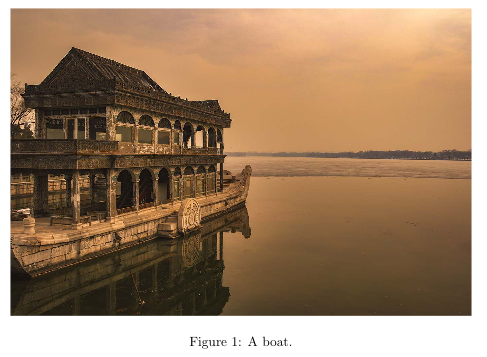
\includegraphics[width=\linewidth]{source/boat.jpg}
		\caption{A boat.}
		\label{fig:boat1}
	\end{figure}
	
	Figure \ref{fig:boat1} shows a boat.
	
	\begin{figure}[!ht]
		\centering
		\begin{subfigure}[b]{0.4\linewidth}
			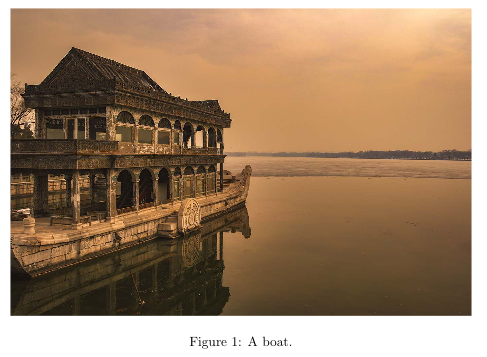
\includegraphics[width=\linewidth]{source/boat.jpg}
			\caption{Boat.}
		\end{subfigure}
		\begin{subfigure}[b]{0.4\linewidth}
			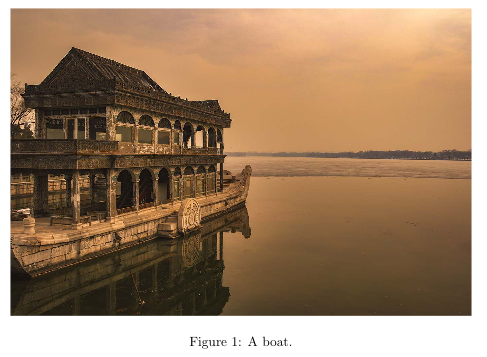
\includegraphics[width=\linewidth]{source/boat.jpg}
			\caption{More Boat.}
		\end{subfigure}
		\caption{The same boat. Two times.}
		\label{fig:coffee}
	\end{figure}
	
	
	\subsection{Sub-subsection}
	
	\paragraph{Paragraph}
	More random text.
	
	\subparagraph{Subparagraph}
	More random text.
	
\end{document}